\documentclass[a4paper]{article}

\usepackage{physics}
\usepackage{pdfpages}
\usepackage{tikz}
\usetikzlibrary{matrix,shapes,arrows,positioning,chains}
\usepackage{lscape}
\usepackage[english]{babel}
\usepackage[utf8]{inputenc}
\usepackage{amsmath}
\usepackage[top=1in, bottom=1.25in, left=1in, right=1in]{geometry}
\usepackage{fancyhdr}
\setlength{\headheight}{15.2pt}
\pagestyle{fancy}
\usepackage{hyperref}
\usepackage{float}
\usepackage{graphicx}
\usepackage{caption}
\usepackage{subcaption}
\usepackage{wrapfig}
\usepackage{color}

\newcommand{\HRule}{\rule{\linewidth}{0.5mm}}

\lhead{Simon Hudson}
\chead{PHYC30012}
\rhead{10-10-2016}

\begin{document}

\begin{center}
\textsc{\Large PHYC30012 Computational Physics}\\[0.3cm]

\HRule \\[0.4cm]

{\LARGE \bfseries Project 4 - Monte-Carlo study of the 2D Ising model \\[0.4cm] }
{\Large 10th October 2016 \\}

\HRule \\[0.3cm]

{\large Simon Hudson 767507\\[0.5cm]}

\end{center}

\section{Introduction}
This project deals with the thermodynamics of the ferromagnetic Ising Model - a 2D array of spins with simple nearest neighbour interactions \cite{Manual}. This model is of interest because it displays a phase transition from disorder $\rightarrow$ order at a critical temperature of $\beta_c$=0.4407. This comes from the exact solution in the large lattice limit by L. Onsager.\\

\section{The 2D ferromagnetic Ising model}\label{2D_ferr_mag_I_model}
The Ising model is defined on a lattice of $N_s=N_x \times Ny$ sites, where $N_x$ and $N_y$ are the number of sites in the x and y directions respectively. The coordinates of a lattice site are $\alpha=(i,j)$ and the spin at site $\alpha$ is $\sigma_{i,j}^{z}$. The configuration of the $N_s$ spins on the lattice is labelled by $\underline{\sigma}^z$.\\

\section{The phase transition}\label{Phase_trans}
Starting from a ``hot'' start, in which the magnetic spins are randomised, the system exhibits a phase change from disorder to order at a certain critical temperature $\beta_c$. This is because the system reaches a certain ``critical mass'' or tipping point, at which small changes in beta yield a large number of sites needing to be flipped, according to the Metropolis algorithm in section \ref{Metro_algo}. As beta increases, the spins in the system slowly flip until there are large numbers of them which are poised to help their neighbours do so. Then, all at once, large numbers of them begin to satisfy the conditions to flip, resulting in a rapid wholesale transition of spins, resulting in a rapid phase change to where most spins are aligned.

\section{The Monte-Carlo method}\label{Monte-Carlo}
The Monte-Carlo method is advantageous when it comes to calculating ensemble averages of physical quantities because it allows one to evaluate, at least approximately, integrals or sums of many variables that would be impossible by quadrature or direct evaluation. The real power of the Monte-Carlo method comes when it is used in conjunction with a carefully chosen \emph{weight} function, w(x). For a given function f(x), the Monte-Carlo procedure is to now sample the ratio f/w over the interval [0,1]. If w(x) is chosen such that it mimics the behaviour of f(x), then the ratio f/w will be relatively flat, the standard deviation of the evaluations will be small, and the accuracy of the method will be much improved.\\

\section{The Metropolis algorithm}\label{Metro_algo}
The Metropolis algorithm is commonly used in Monte-Carlo computations. It essentially guides a random walker through the space of points $\overrightarrow{x\,}$ such that successive points in the walk are approximately distributed according to the distribution $w(\overrightarrow{x\,})$ using the following methodology. The walker is at point $\overrightarrow{x\,}_n$ and chooes a trial point $\overrightarrow{x\,}_t$ at random and calculates the ratio:
\begin{align}
	r\equiv\frac{w(\overrightarrow{x\,}_t)}{w(\overrightarrow{x\,}_n)}
\end{align}
\noindent Then:
\begin{itemize}
	\item If $r>1$, the step to $\overrightarrow{x\,}_t$ is accepted and thus the next point in the set is $\overrightarrow{x\,}_{n+1}=\overrightarrow{x\,}_t$
	\item If $r<1$, the step is accepted with probability r, ie for a uniform random number $\eta$ in [0,1]:
	\begin{itemize}
		\item If $r>\eta$ accept $\overrightarrow{x\,}_t$ ie $\overrightarrow{x\,}_{n+1}=\overrightarrow{x\,}_t$.
		\item If $r<\eta$ reject $\overrightarrow{x\,}_t$ and try another random trial point.
	\end{itemize}
\end{itemize}

\noindent The set of points $\{\overrightarrow{x\,}_n\}$ are then used in the Monte-Carlo evaluation.\\

\noindent In this case, the calculation of r is done using the contribution $\epsilon$ to the lattice energy of each lattice point $(i,j)$ with spin $\sigma_{i,j}$. This contribution is given by:
\begin{align}
	\epsilon=-J\sigma_{i,j}\left[\sigma_{i-1,j}+\sigma_{i,j+1}+\sigma_{i+1,j}+\sigma_{i,j-1}\right] \label{Eq_Metr_Alg_E}
\end{align}
In our case we will take $J=1$. If we flipped the spin of this lattice point, then the contribution to the total lattice energy E of this trial configuration will be $-\epsilon$, ie $\Delta E=-2\epsilon$. Thus this flip will be accepted:
\begin{itemize}
	\item If the energy is lowered by the flip ie $\Delta E<0$, or
	\item If $e^{-\beta\Delta E}>\eta$, where $\eta$ is a random number uniformly distributed in [0,1]
\end{itemize}

\section{Statistics}\label{Stats}
We wish to calculate the magnetisation of the lattice for different values of $\beta$, and observe the phase change at the critical temperature. However for anything above small lattice sizes, the number of calculations involved is huge. Therefore we need to use the Monte-Carlo procedure with the Metropolis algorithm to generate configurations according to the probability distribution, $P(\underline{\sigma}^z)$.\\

\noindent The magnetisation of the lattice $M(\underline{\sigma}^z)$ in configuration $\underline{\sigma}^z$ is the sum over all the spins:

\begin{align}
	M(\underline{\sigma}^z)=\frac{\abs*{\sum_{\alpha}\sigma_\alpha}}{N_x \times N_y}
\end{align}

\noindent After generating a set of N configurations by the Metropolis algorithm, then the ensemble average of the magnetisation (the observed value) is approximately given by the Monte-Carlo average:
\begin{align}
	M=\left<M\right>\approx\frac{1}{N}\sum_{k=1}^{N}M_k \label{M_C_avge}
\end{align}
where $M_k$ is the magnetisation in the $k^{th}$ configuration. The Monte-Carlo measurement of the magnetisation is then given by:
\begin{align}
	M=\left<M\right>\pm\sigma_M
\end{align}
where, if the configurations are statistically independent, the bias-corrected variance is given by:
\begin{align}
	\sigma^2_{M-1}=\frac{1}{N-1}\sum_{k=1}^{N}(M_k-\left<M\right>)^2 \label{M_C_var}
\end{align}

\begin{align}
	\approx\left<M^2\right>-\left<M\right>^2
\end{align}

\clearpage
\section{Method and results}\label{Method_results}
\begin{enumerate}
	\item The procedure outlined in the flowchart of figure \ref{Fig_flowchart} was implemented. All input values are set at the top of the code using #define.
	\begin{enumerate}
		\item The Knuth procedure involves the following. For each of the entries in the 1D Knuth array, say at index i, choose a number from the uniform distribution on [0,1], multiply it by the size of the array, and convert to an integer, j. Then exchange the current entry at index i with the entry at index j. This gives the selection for the Metropolis algorithm of equation \ref{Eq_Metr_Alg_E}.
		\item Using a software profiler, it was found that the Knuth algorithm was a bottleneck in speed of the program. With further testing and optimisation of this function, sufficient efficiency was achieved that allowed larger lattices such as 500x500 to 1500x1500.
	\end{enumerate}
	\item Repeated Metropolis sweeps are required after changing the temperature and between measurements because configurations obtained in consecutive sweeps may be somewhat correlated. After starting in either ``hot'' or ``cold'' mode, a number of sweeps are required to ``thermalise'' the lattice before a measurement is taken, ie allowing the lattice to acclimatise to the experimental ``temperature'' to which it is exposed. For example, if a lattice is started in the ``cold'' configuration, but then put into an experimental setup where beta is supposed to be low (meaning high temperature), it will take a number of sweeps before it has acclimatised to this temperature. Here, we accommodate for this by allowing 100 sweeps after each temperature change.
	
	\item Random spins are used for a ``hot'' start, because this is the state of the system for higher temperatures. Because of the higher thermal energy of the system, the spins are not aligned in one particular direction, but rather randomly distributed throughout the material. The higher the temperature, the more the system tends toward disorder and a random distribution of spin, which leads to a magnetisation that tends to zero. Aligned spins are used for a ``cold'' start because as the temperature tends towards zero, there is less and less energy in the system, so the spins tend to line up in one direction. This configuration minimises the energy of the system overall, and leads to a magnetisation tending to one.
\end{enumerate}

\clearpage
\tikzstyle{startstop} = [rectangle, rounded corners, minimum width=3cm, minimum height=1cm,text centered, draw=black, fill=red!30]
\tikzstyle{io} = [trapezium, trapezium left angle=70, trapezium right angle=110, minimum width=3cm, minimum height=1cm, text centered, draw=black, fill=blue!30]
\tikzstyle{process} = [rectangle, minimum width=3cm, minimum height=1cm, text centered, draw=black, fill=orange!30]
\tikzstyle{decision} = [diamond, minimum width=3cm, minimum height=1cm, text centered, draw=black, fill=green!30]
\tikzstyle{arrow} = [thick,->,>=stealth]

\begin{figure}
	\centering
	\caption{Flowchart for complete program operation.} \label{Fig_flowchart}
	\begin{tikzpicture} [
		start chain,
		node distance=3mm, 
		every node/.style={
			fill=blue!20,
			inner sep=2mm
		}, 
		inner sep=5pt,
		text width=7cm,
		auto
	]
		\node (start) [
			startstop,
			draw,
			on chain=going below,
			join
		] {
			Start
		};
		\node (accept) [
			io,
			below of=start,
			draw,
			on chain=going below,
			join
		] {
			Accept input values:
			\begin{itemize}
				\item $N_x$ and $N_y$ for x and y lattice sides
				\item type of start (``hot'' or ``cold'')
				\item total number of sweeps
				\item number of sweeps between measurements
			\end{itemize}
			};
		\node (create) [
			process,
			below of=accept,
			draw,
			on chain=going below,
			join
		] {
			\begin{itemize}
				\item Create 2D lattice and initialise spins:
				\begin{itemize}
					\item randomly for hot start, or 
					\item aligned for cold start
				\end{itemize}
				\item Create 1D array to be used for Knuth procedure of efficiently randomly selecting all lattice sites for examination
			\end{itemize}
		};
		\node (thermalise) [
			process,
			below of=create,
			draw,
			on chain=going below,
			join
		] {
			Sweep 100 times using Knuth procedure to randomise selections, and using Metropolis algorithm to conditionally flip spins as per equation \ref{Eq_Metr_Alg_E}, to thermalise lattice for this value of $\beta$
		};
		\node (measure) [
			process,
			below of=thermalise,
			draw,
			on chain=going below,
			join
		] {
			Take 10 measurements of magnetisation, sweeping 10 times in between each one to thermally decorrelate lattice
		};
		\node (variance) [
			process,
			below of=measure,
			draw,
			on chain=going below,
			join
		] {
			Calculate the variance of the magnetisation measurements
		};
		\node (dec-mag-domains) [
			process,
			below of=variance,
			draw,
			on chain=going below,
			join
		] {
			If the beta value at critical temperature, plot ferro-magnetic domains
		};
		\node (plot-mag-beta) [
			process,
			below of=dec-mag-domains,
			draw,
			on chain=going below,
			join
		] {
			Plot the lattice magnetisation versus beta, including error bars
		};
		\node (stop) [
			startstop,
			below of=plot-mag-beta,
			draw,
			on chain=going below,
			join
		] {
			Stop
		};
			
		\draw [arrow] (start) -- (accept);
		\draw [arrow] (accept) -- (create);
		\draw [arrow] (create) -- (thermalise);
		\draw [arrow] (thermalise) -- (measure);
		\draw [arrow] (measure) -- (variance);
		\draw [arrow] (variance) -- (dec-mag-domains);
		\draw [arrow] (dec-mag-domains) -- (plot-mag-beta);
		\draw [arrow] (plot-mag-beta) -- (stop);
		
	\end{tikzpicture}
\end{figure}

\clearpage
\begin{figure}[ht!]
	\centering
	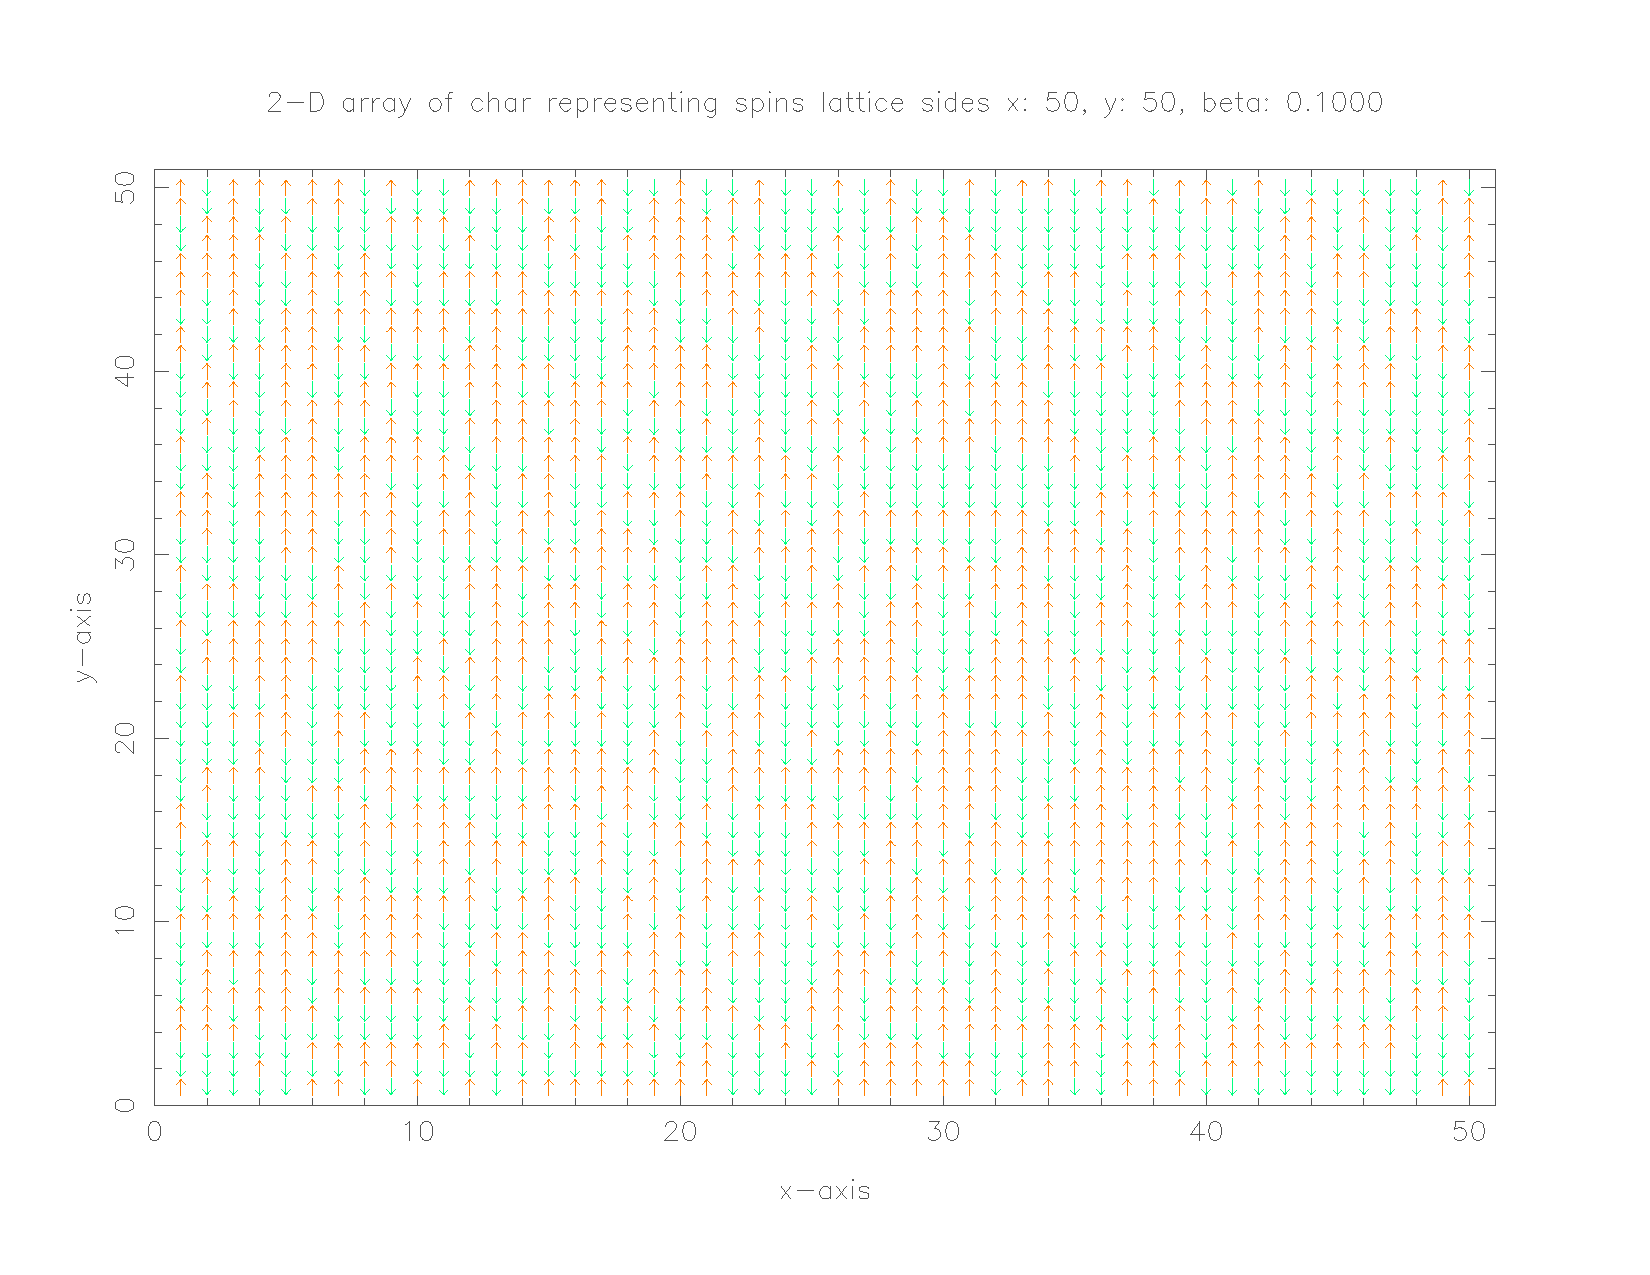
\includepdf[pages=1]{plots/proj4plot50.pdf}
	\caption{Plot of 2D character array representing lattice spins for ``hot'' start.}\label{Fig_lattice_plot}
\end{figure}

\clearpage
\begin{enumerate}
	\setcounter{enumi}{5}
	\item A example plot of the state of the lattice for a lattice size of 50x50 using cpgplot for a ``hot'' start is shown in figure \ref{Fig_lattice_plot}.

	\item The results for the absolute value of magnetisation versus $\beta$, including error bars for standard deviation, for various lattice sizes are plotted in figures \ref{Fig_mag_plot_64_hot} to \ref{Fig_mag_plot_1500_2}. Magnetisation is calculated using equation \ref{M_C_avge} and standard deviation using equation \ref{M_C_var}. The lattice sizes, number of measurements of magnetisation, and measurement sweep separation are noted in figure titles. The critical temperatures marked on the plots was taken from the place at which the standard deviation was greatest, since this is the region of the highest rate of change, resulting in the highest spread of values. This corresponds to the region of the phase change from disorder $\rightarrow$ order, since there is a maximal rate of change of magnetisation at this point.
	
	\item Both ``hot'' (figure \ref{Fig_mag_plot_64_hot}) and ``cold' (figure \ref{Fig_mag_plot_64_cold})' starts were investigated. We can see that for the hot start, the curve tends to be smoother with less backtracking. This is to be expected, since for a hot start, the lattice is already more thermalised to the low beta starting temperature. 
	
	\item The critical temperature for the phase transition for different lattice sizes was discovered to be very close to the analytic value of 0.4407 obtained by Onsager. This corresponds to a temperature of $T_c=3.191978\times10^{22} K$.
	
	\item The features of the plot that change with lattice size are as follows:
	\begin{enumerate}
		\item In general the larger the lattice becomes, the smoother the curve becomes. That is, as beta changes, the magnetisation of the lattice increases in a more uniform and predictable way. This is to be expected because more data points are being used in the calculations.
		\item Also, as the lattice becomes larger, the size of the standard deviation error bars decreases. This is also to be expected since for larger lattices, the variance in measurements of magnetisation should be lower because the lattice is more uniform and differences between nearest neighbours will be smaller.
		\item For some lattice sizes (specifically 250x250, 450x450, 550x550, 650x650 and 1500x1500), the magnetisation never reaches its expected value of one. This is saying that as the temperature drops, the lattice never completes its phase change and not all of the spins end up lining up. This might be due to the fact that as the lattice gets larger, it takes longer and longer for the lattice to thermalise, and the effects of the temperature changes are not able to be felt for each value of $\beta$.
		\item Also, for the large lattices where the magnetisation does eventually reach one (specifically 750x750 and 850x850), there was not as sharp a phase change as for the smaller lattices. This can be explained by the same mechanism - the lattice takes longer to thermalise with each temperature change, and hence all changes in spin take longer to propagate.
		\item After some investigation, the lattice size for which this started to occur was around 175x175 (see figure \ref{Fig_mag_plot_175_sweeps_1100}). For this reason, the same lattice size was investigated using:
			\begin{enumerate}
				\item An increased number of measurements ie for each value of $\beta$, taking 100 measurements of magnetisation, each separated by 10 sweeps (see figure \ref{Fig_mag_plot_175_sweeps_11000_10sep}). Here $\beta_c=0.43$.
				\item An increased number of sweeps ie for each value of $\beta$, taking 10 measurements of magnetisation, each separated by 100 sweeps (see figure \ref{Fig_mag_plot_175_sweeps_11000_100sep}). Here $\beta_c=0.45$.
		 	\end{enumerate}
	 	In both of these cases, the expected behaviour of a sharp phase change is now there. However it occurs at different values of $\beta$ in each case. This is because of the way we have defined our experimental $\beta_c$ (the region of maximum standard deviation). If we are doing more sweeps between measurements, the lattice has more time to thermalise for each new value of $\beta$, and the standard deviation will be lower.\\
	 	
	 	When repeated for the next lattice size 250x250 that exhibited the unexpected absence of phase change, taking 10 measurements each separated by 100 sweeps, the expected phase change is now present (see figure \ref{Fig_mag_plot_250_sweeps_11000_100sep}). Therefore we conclude that larger lattices need more sweeps to thermalise to each new $\beta$.
	\end{enumerate}

	\item Scatter plots of the lattice for lattice sizes from 250x250 to 1500x1500 for a beta value of 0.44 (closest to Onsager's analytic value of 0.4407) are shown in figures \ref{Fig_mag_plot_250_1} to \ref{Fig_mag_plot_1500_1}. The lattice sizes are noted in the figure titles. It can clearly be seen that ferromagnetic domains form as the lattice goes from low $\beta$ (high temperature) to high $\beta$ (low temperature) undergoes the phase change. \label{Scatter_plots}
		\begin{enumerate}
			\item The size, shape and distribution of the ferro-magnetic domains is roughly constant as lattice size increases. 
			\item To conduct a more detailed analysis, it would be preferable to examine the ferro-magnetic domains at the exact point of phase change. This would require a different programming approach which would require more computational power, and is hence beyond the scope of this project.
		\end{enumerate}

	\item Errors
		\begin{itemize}
			\item Statistical error in experimental measurements are caused by unknown and unpredictable changes in the experiment. They tend to form a Gaussian normal distribution \cite{Rand_v_syst_err}. In this project, these consist of:
				\begin{itemize}
					\item Errors in the magnetisation measurements between sweeps.
				\end{itemize}
			These can be decreased by increasing the number of magnetisation measurements taken. However, this may increase the systematic error, since the number of sweeps between measurements will decrease, and hence each measurement may be more correlated.
			\item Systematic error, however, is predictable and typically constant or proportional to the true value \cite{Syst_Wiki}. Systematic errors are often due to a problem which persists throughout the entire experiment. Here they are represented by:
				\begin{itemize}
					\item  Error due to correlation between successive magnetisation measurements, 
					\item  Error due to a finite lattice size (as compared to the infinite lattice limit)
		 		\end{itemize}
	 		These can be decreased by increasing the number of sweeps between measurements, and increasing lattice size. However, as has been shown in point \ref{Scatter_plots}, adjustment of other experimental parameters may also be therefore required.
		\end{itemize}
\end{enumerate}

\clearpage
\begin{figure}[ht!]
	\centering
	\includepdf[pages=2]{plots/proj4plot64-hot.pdf}
	\caption{Plot of magnetisation vs. $\beta$ with 10 measurements per value of $\beta$, each separated by 10 sweeps, ``hot'' start .}\label{Fig_mag_plot_64_hot}
\end{figure}

\clearpage
\begin{figure}[ht!]
	\centering
	\includepdf[pages=2]{plots/proj4plot64-cold.pdf}
	\caption{Plot of magnetisation vs. $\beta$ with 10 measurements per value of $\beta$, each separated by 10 sweeps, ``cold'' start .}\label{Fig_mag_plot_64_cold}
\end{figure}

\clearpage
\begin{figure}[ht!]
	\centering
	\includepdf[pages=2]{plots/proj4plot100.pdf}
	\caption{Plot of magnetisation vs. $\beta$ with 10 measurements per value of $\beta$, each separated by 10 sweeps.}\label{Fig_mag_plot_100}
\end{figure}

\clearpage
\begin{figure}[ht!]
	\centering
	\includepdf[pages=2]{plots/proj4plot150.pdf}
	\caption{Plot of magnetisation vs. $\beta$ with 10 measurements per value of $\beta$, each separated by 10 sweeps.}\label{Fig_mag_plot_150}
\end{figure}

\clearpage
\begin{figure}[ht!]
	\centering
	\includepdf[pages=2]{plots/proj4plot175sweeps1100.pdf}
	\caption{Plot of magnetisation vs. $\beta$ with 10 measurements per value of $\beta$, each separated by 10 sweeps.}\label{Fig_mag_plot_175_sweeps_1100}
\end{figure}

\clearpage
\begin{figure}[ht!]
	\centering
	\includepdf[pages=2]{plots/proj4plot175sweeps11000-10sep.pdf}
	\caption{Plot of magnetisation vs. $\beta$ with 100 measurements per value of $\beta$, each separated by 10 sweeps.}\label{Fig_mag_plot_175_sweeps_11000_10sep}
\end{figure}

\clearpage
\begin{figure}[ht!]
	\centering
	\includepdf[pages=2]{plots/proj4plot175sweeps11000-100sep.pdf}
	\caption{Plot of magnetisation vs. $\beta$ with 10 measurements per value of $\beta$, each separated by 100 sweeps.}\label{Fig_mag_plot_175_sweeps_11000_100sep}
\end{figure}

\clearpage
\begin{figure}[ht!]
	\centering
	\includepdf[pages=2]{plots/proj4plot250.pdf}
	\caption{Plot of magnetisation vs. $\beta$ with 10 measurements per value of $\beta$, each separated by 10 sweeps.}\label{Fig_mag_plot_250_2}
\end{figure}

\clearpage
\begin{figure}[ht!]
	\centering
	\includepdf[pages=2]{plots/proj4plot250sweeps11000-100sep.pdf}
	\caption{Plot of magnetisation vs. $\beta$ with 10 measurements per value of $\beta$, each separated by 100 sweeps.}\label{Fig_mag_plot_250_sweeps_11000_100sep}
\end{figure}

\clearpage
\begin{figure}[ht!]
	\centering
	\includepdf[pages=2]{plots/proj4plot350.pdf}
	\caption{Plot of magnetisation vs. $\beta$ with 10 measurements per value of $\beta$, each separated by 10 sweeps.}\label{Fig_mag_plot_350_2}
\end{figure}

\clearpage
\begin{figure}[ht!]
	\centering
	\includepdf[pages=2]{plots/proj4plot450.pdf}
	\caption{Plot of magnetisation vs. $\beta$ with 10 measurements per value of $\beta$, each separated by 10 sweeps.}\label{Fig_mag_plot_450_2}
\end{figure}

\clearpage
\begin{figure}[ht!]
	\centering
	\includepdf[pages=2]{plots/proj4plot550.pdf}
	\caption{Plot of magnetisation vs. $\beta$ with 10 measurements per value of $\beta$, each separated by 10 sweeps.}\label{Fig_mag_plot_550_2}
\end{figure}

\clearpage
\begin{figure}[ht!]
	\centering
	\includepdf[pages=2]{plots/proj4plot650.pdf}
	\caption{Plot of magnetisation vs. $\beta$ with 10 measurements per value of $\beta$, each separated by 10 sweeps.}\label{Fig_mag_plot_650_2}
\end{figure}

\clearpage
\begin{figure}[ht!]
	\centering
	\includepdf[pages=2]{plots/proj4plot750.pdf}
	\caption{Plot of magnetisation vs. $\beta$ with 10 measurements per value of $\beta$, each separated by 10 sweeps.}\label{Fig_mag_plot_750_2}
\end{figure}

\clearpage
\begin{figure}[ht!]
	\centering
	\includepdf[pages=2]{plots/proj4plot850.pdf}
	\caption{Plot of magnetisation vs. $\beta$ with 10 measurements per value of $\beta$, each separated by 10 sweeps.}\label{Fig_mag_plot_850_2}
\end{figure}

\clearpage
\begin{figure}[ht!]
	\centering
	\includepdf[pages=2]{plots/proj4plot1500.pdf}
	\caption{Plot of magnetisation vs. $\beta$ with 10 measurements per value of $\beta$, each separated by 10 sweeps.}\label{Fig_mag_plot_1500_2}
\end{figure}




\clearpage
\begin{figure}[ht!]
	\centering
	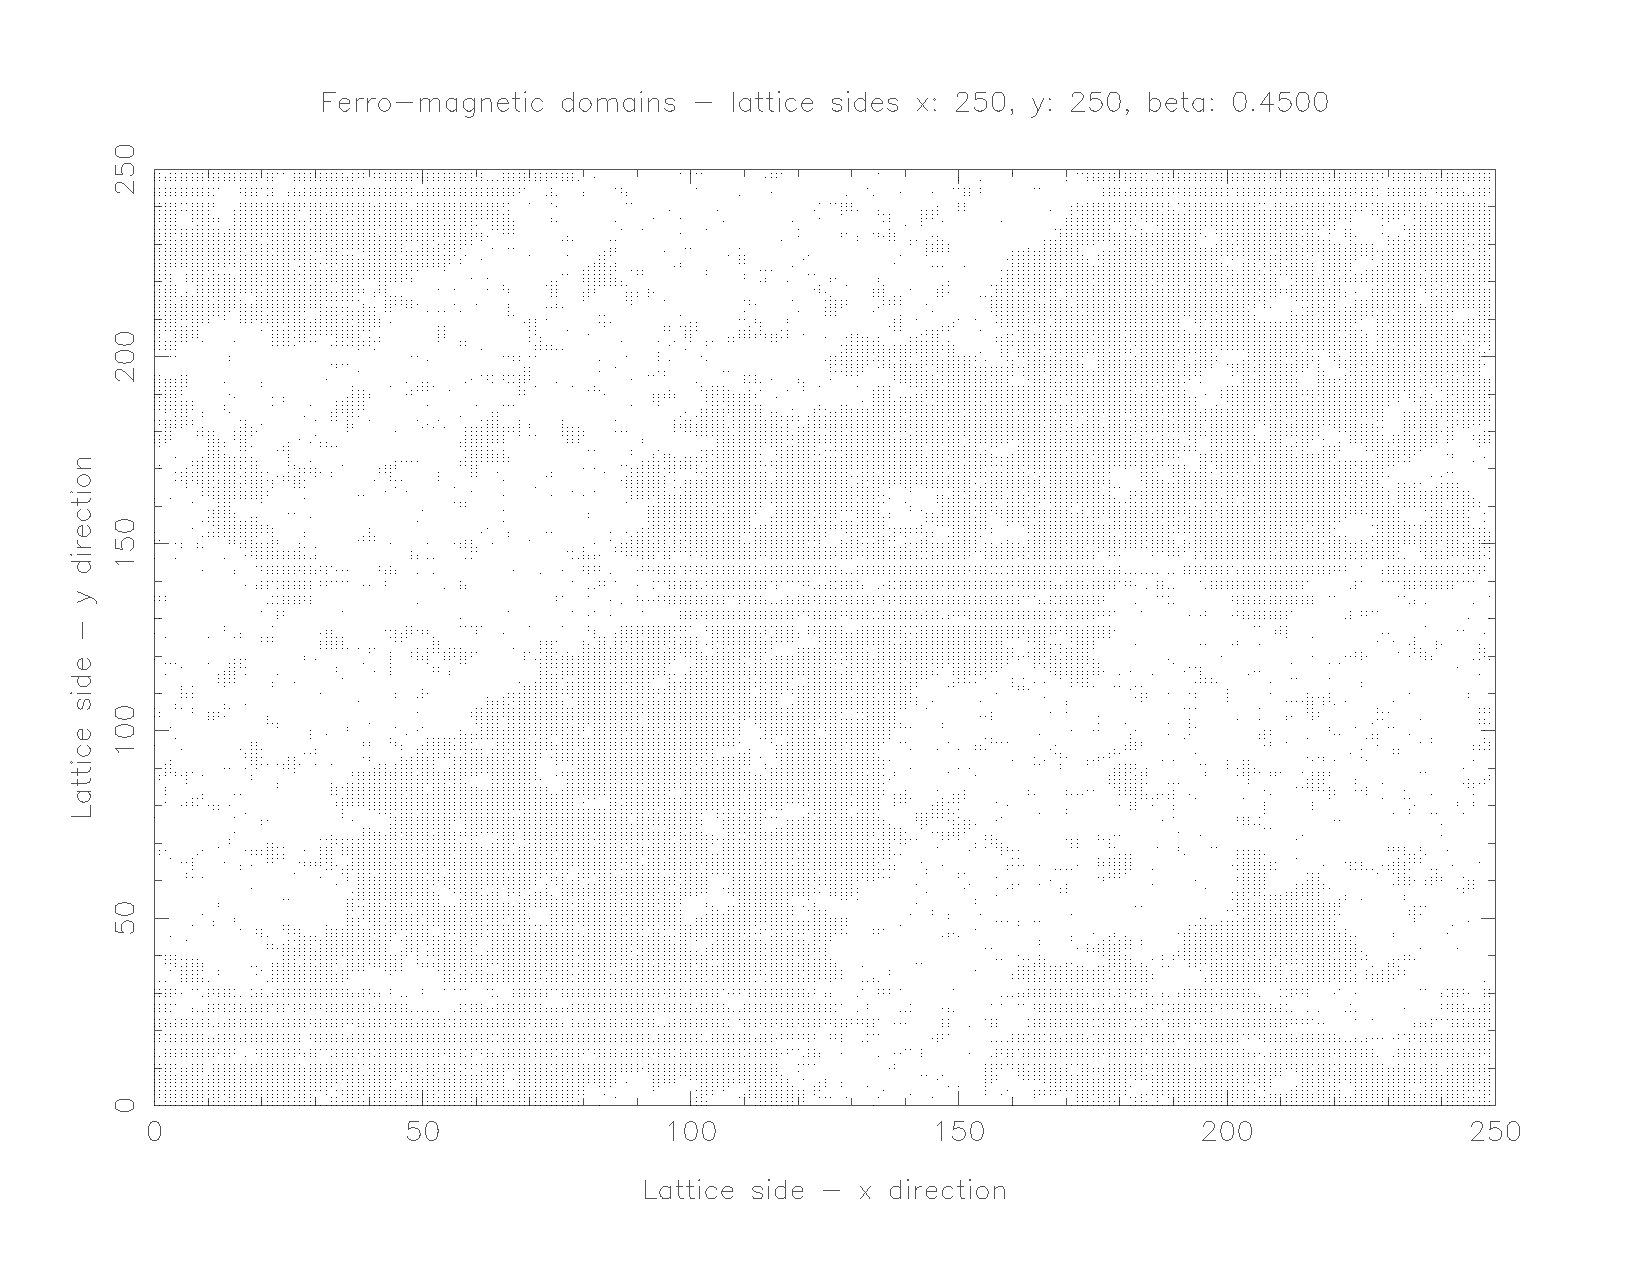
\includepdf[pages=1]{plots/proj4plot250.pdf}
	\caption{Scatter plot of lattice at $\beta\approx0.44$ showing ferro-magnetic domains.}\label{Fig_mag_plot_250_1}
\end{figure}

\clearpage
\begin{figure}[ht!]
	\centering
	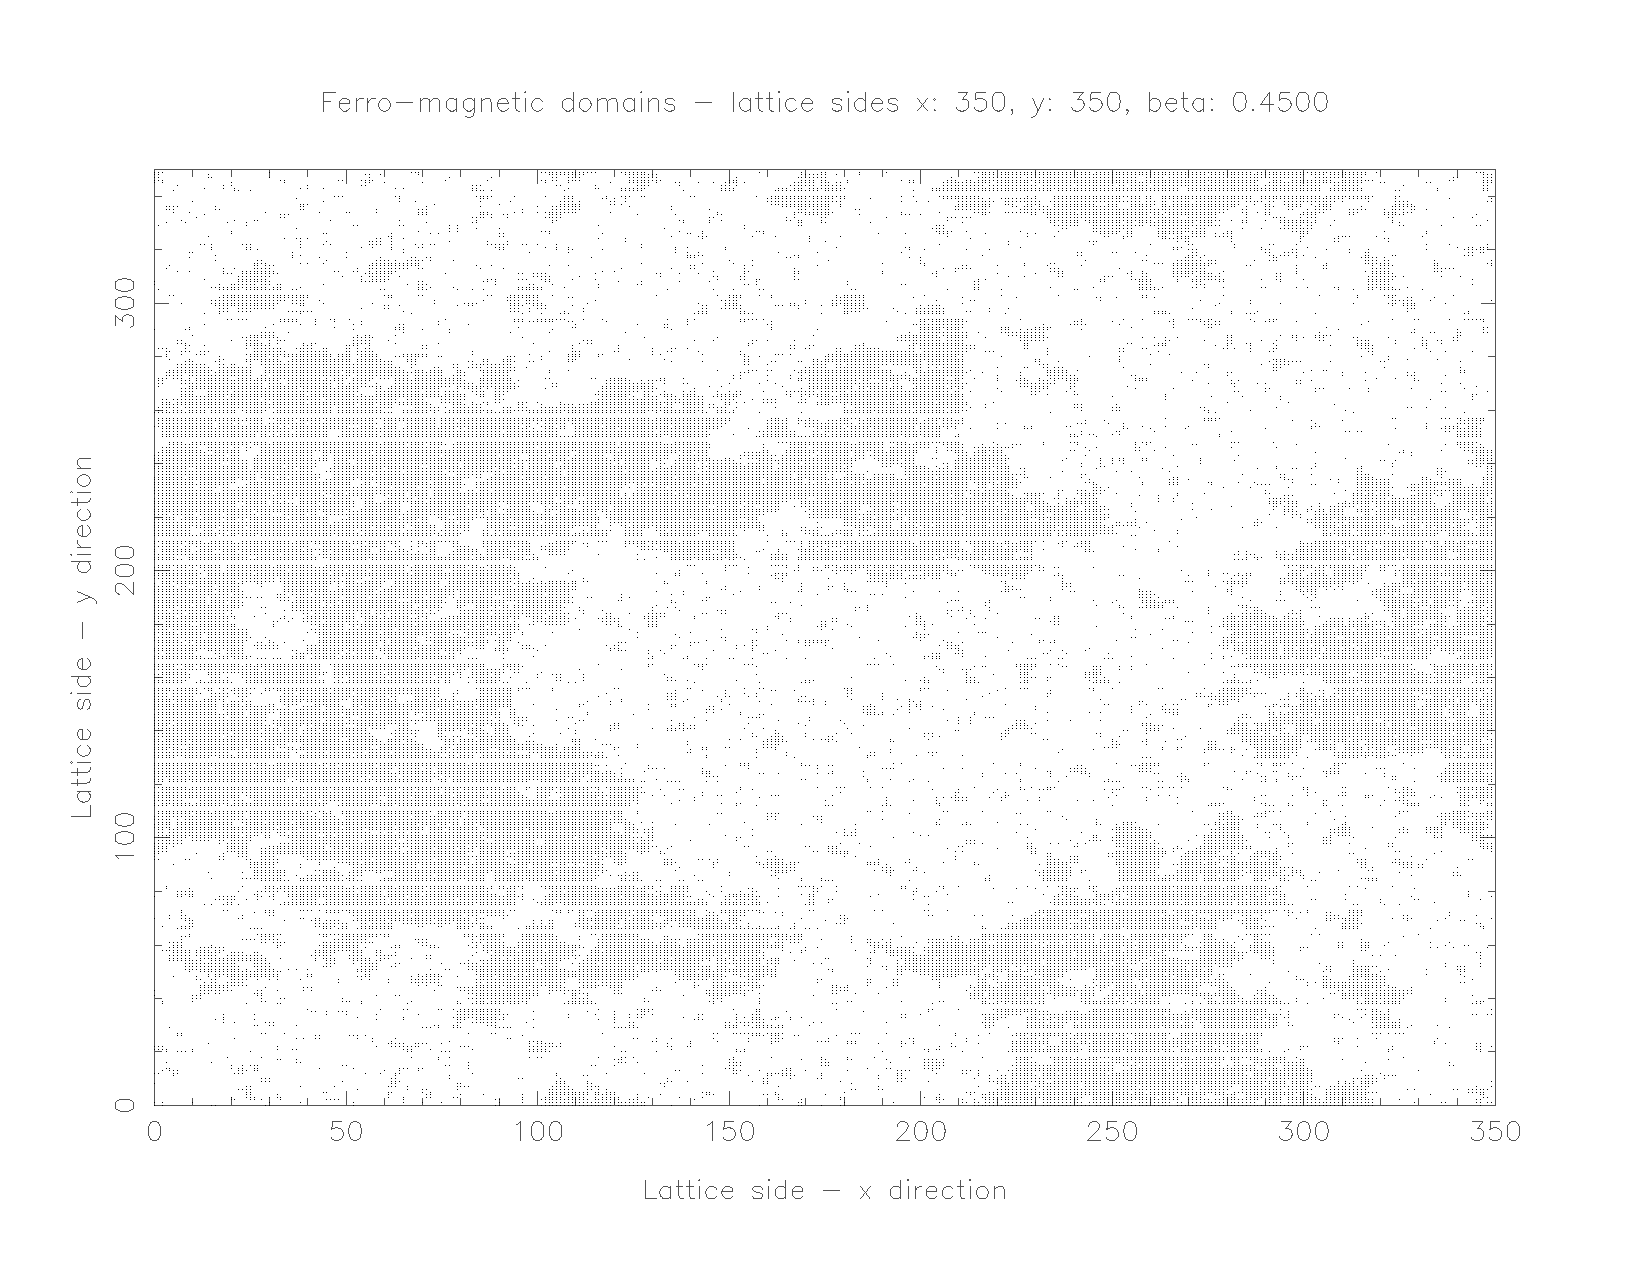
\includepdf[pages=1]{plots/proj4plot350.pdf}
	\caption{Scatter plot of lattice at $\beta\approx0.44$ showing ferro-magnetic domains.}\label{Fig_mag_plot_350_1}
\end{figure}

\clearpage
\begin{figure}[ht!]
	\centering
	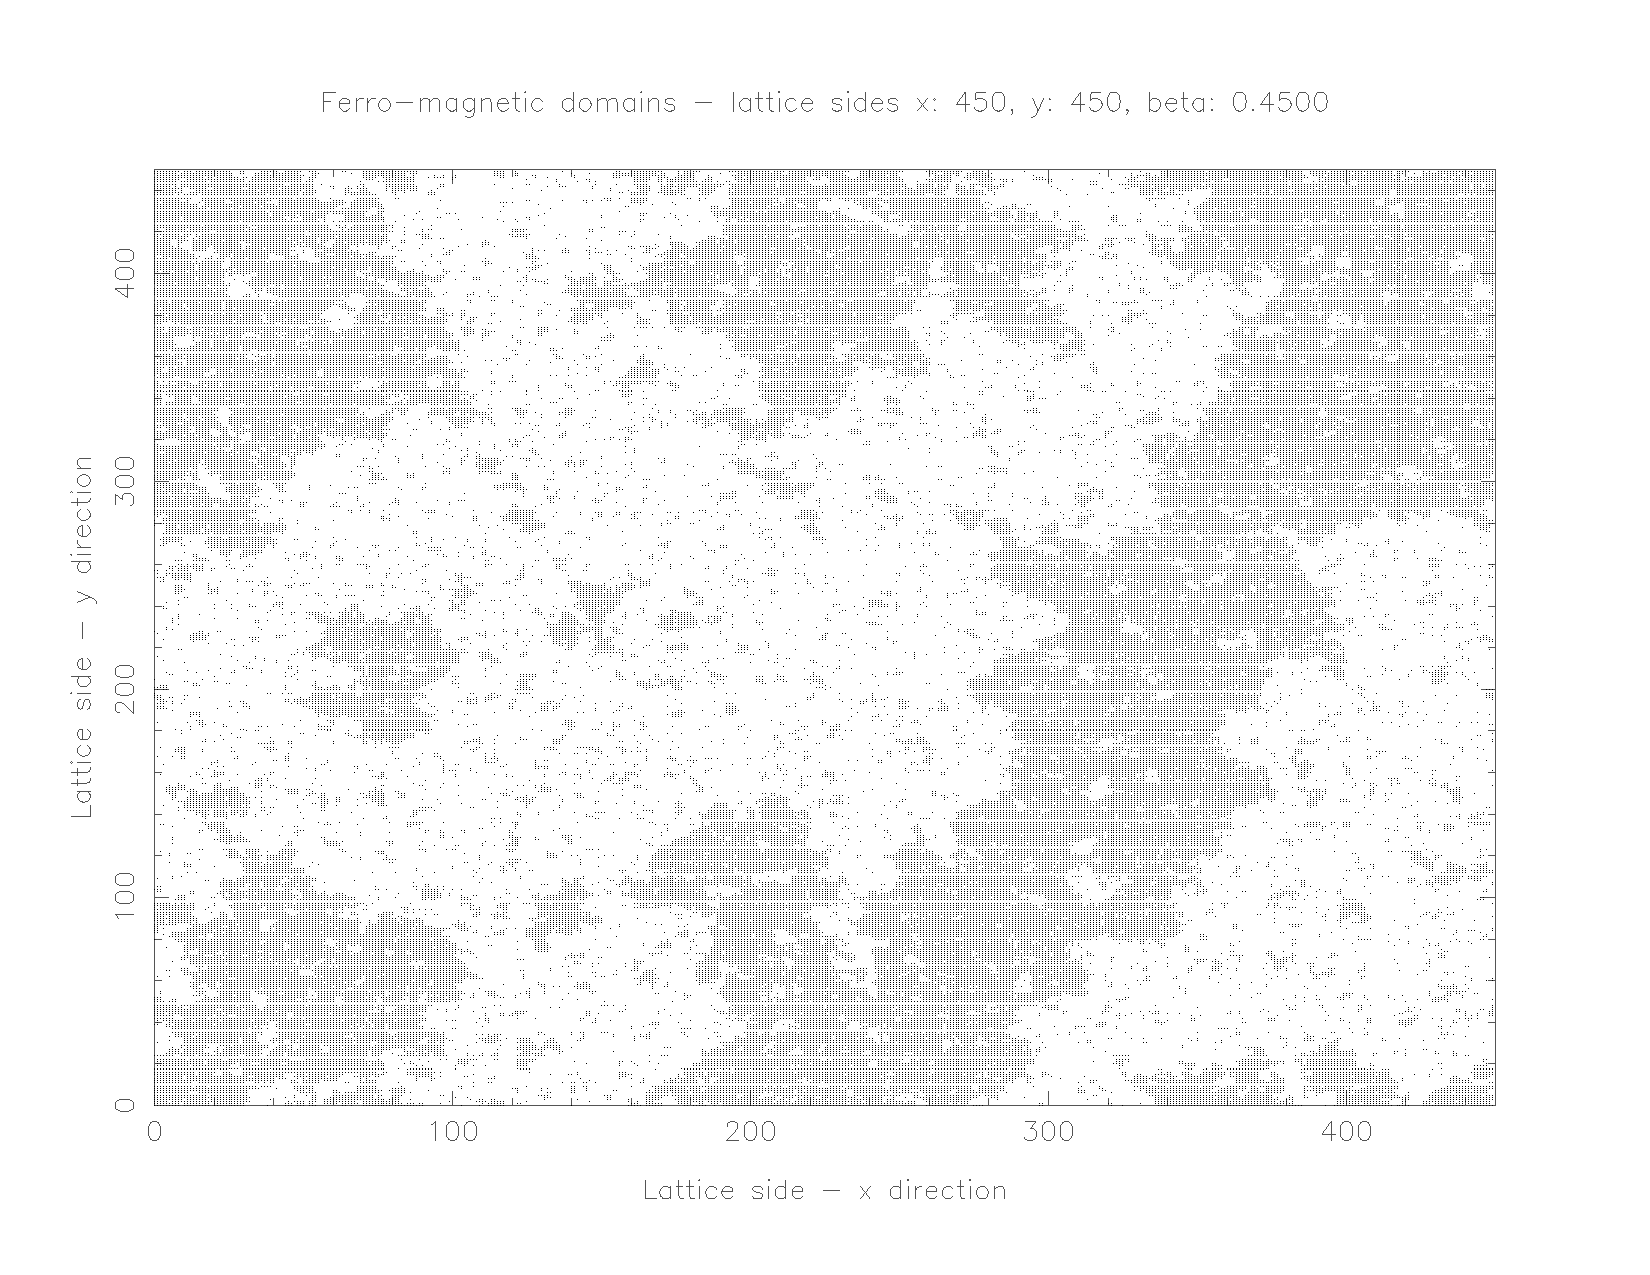
\includepdf[pages=1]{plots/proj4plot450.pdf}
	\caption{Scatter plot of lattice at $\beta\approx0.44$ showing ferro-magnetic domains.}\label{Fig_mag_plot_450_1}
\end{figure}

\clearpage
\begin{figure}[ht!]
	\centering
	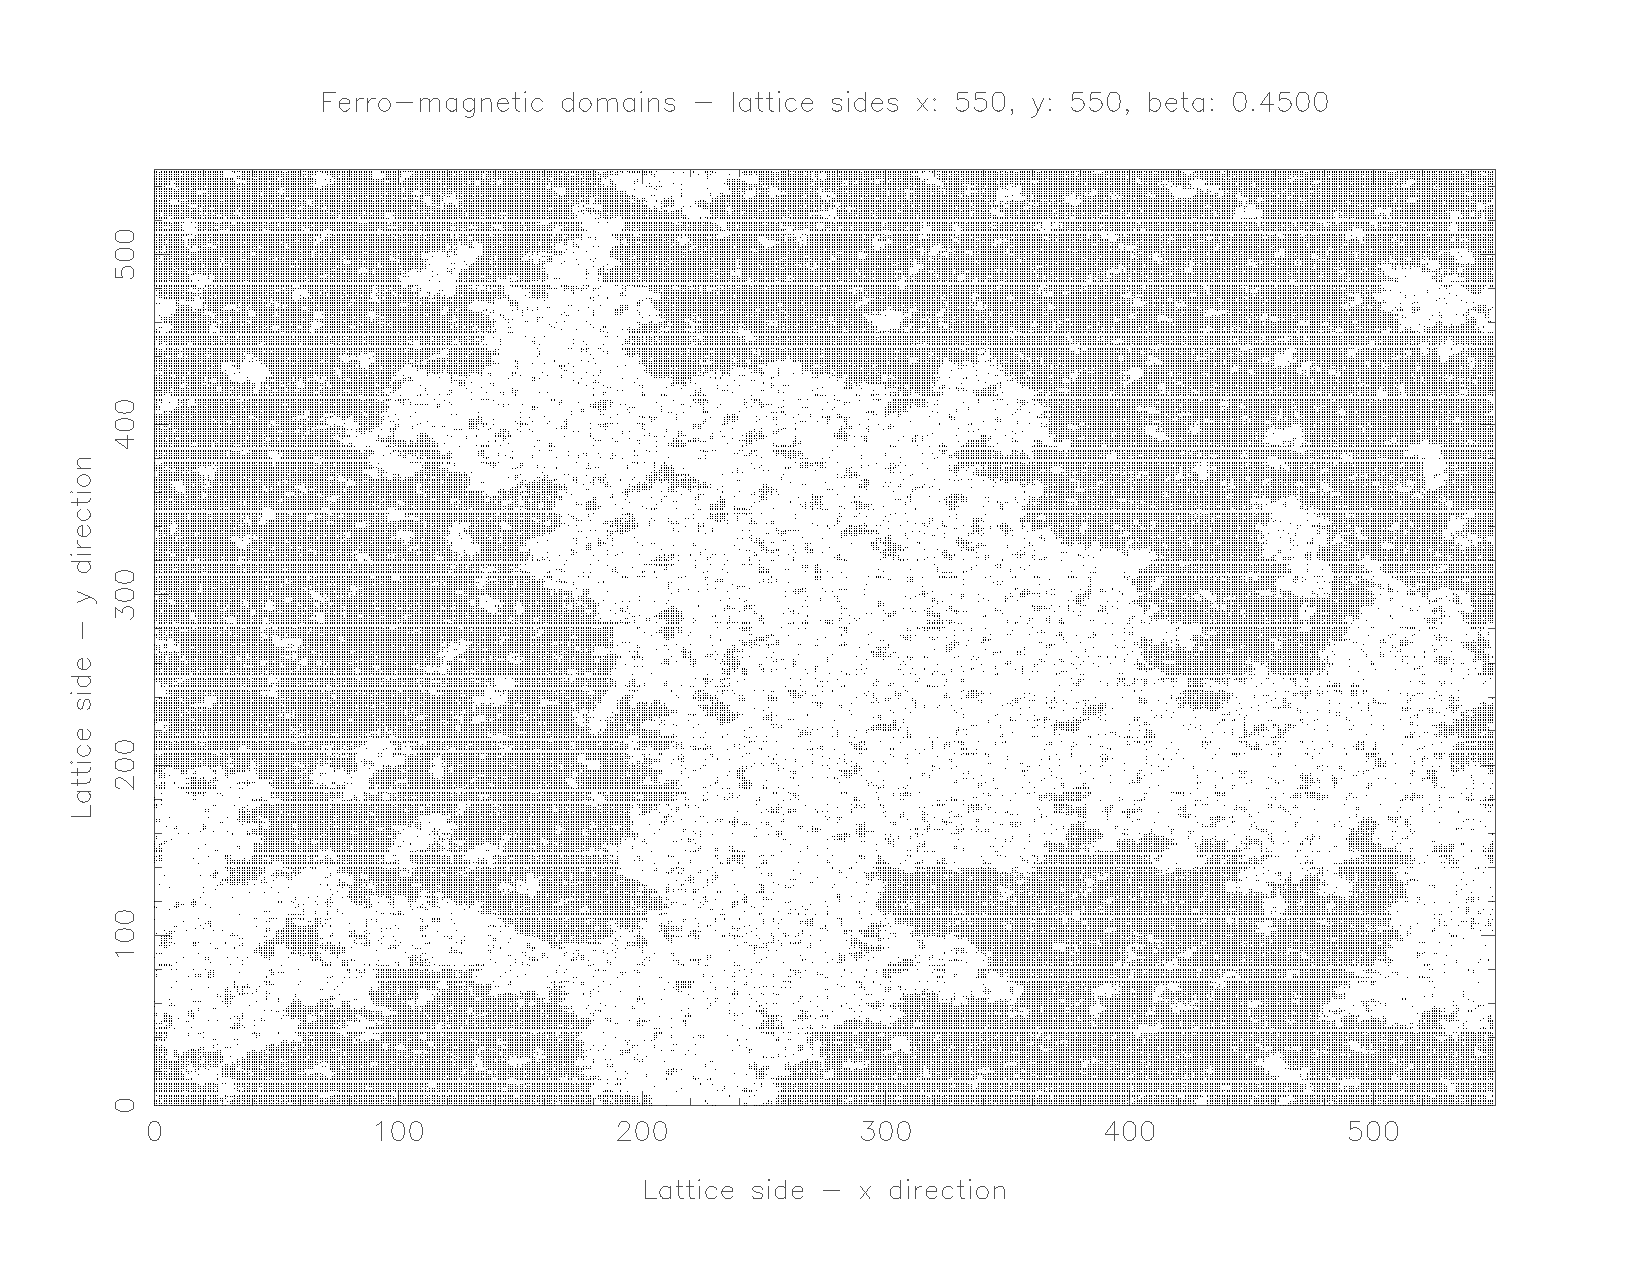
\includepdf[pages=1]{plots/proj4plot550.pdf}
	\caption{Scatter plot of lattice at $\beta\approx0.44$ showing ferro-magnetic domains.}\label{Fig_mag_plot_550_1}
\end{figure}

\clearpage
\begin{figure}[ht!]
	\centering
	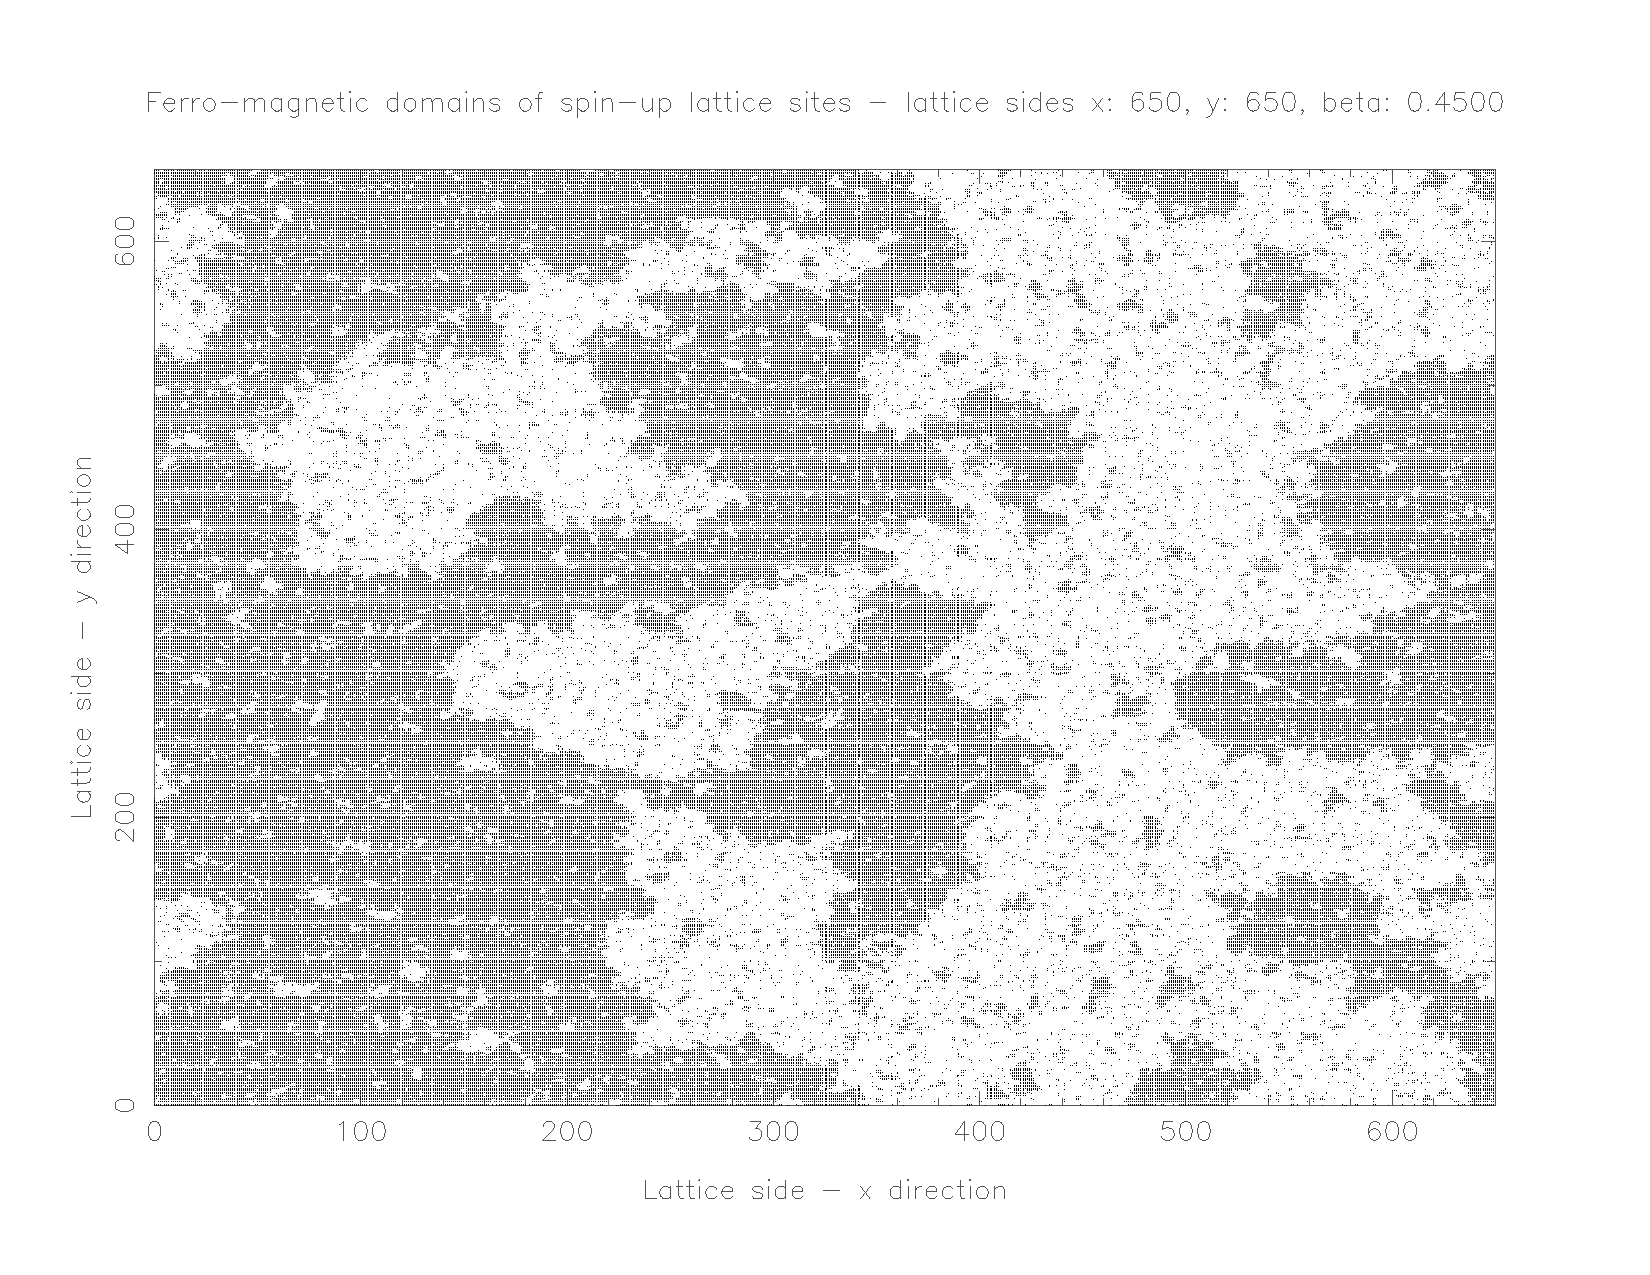
\includepdf[pages=1]{plots/proj4plot650.pdf}
	\caption{Scatter plot of lattice at $\beta\approx0.44$ showing ferro-magnetic domains.}\label{Fig_mag_plot_650_1}
\end{figure}

\clearpage
\begin{figure}[ht!]
	\centering
	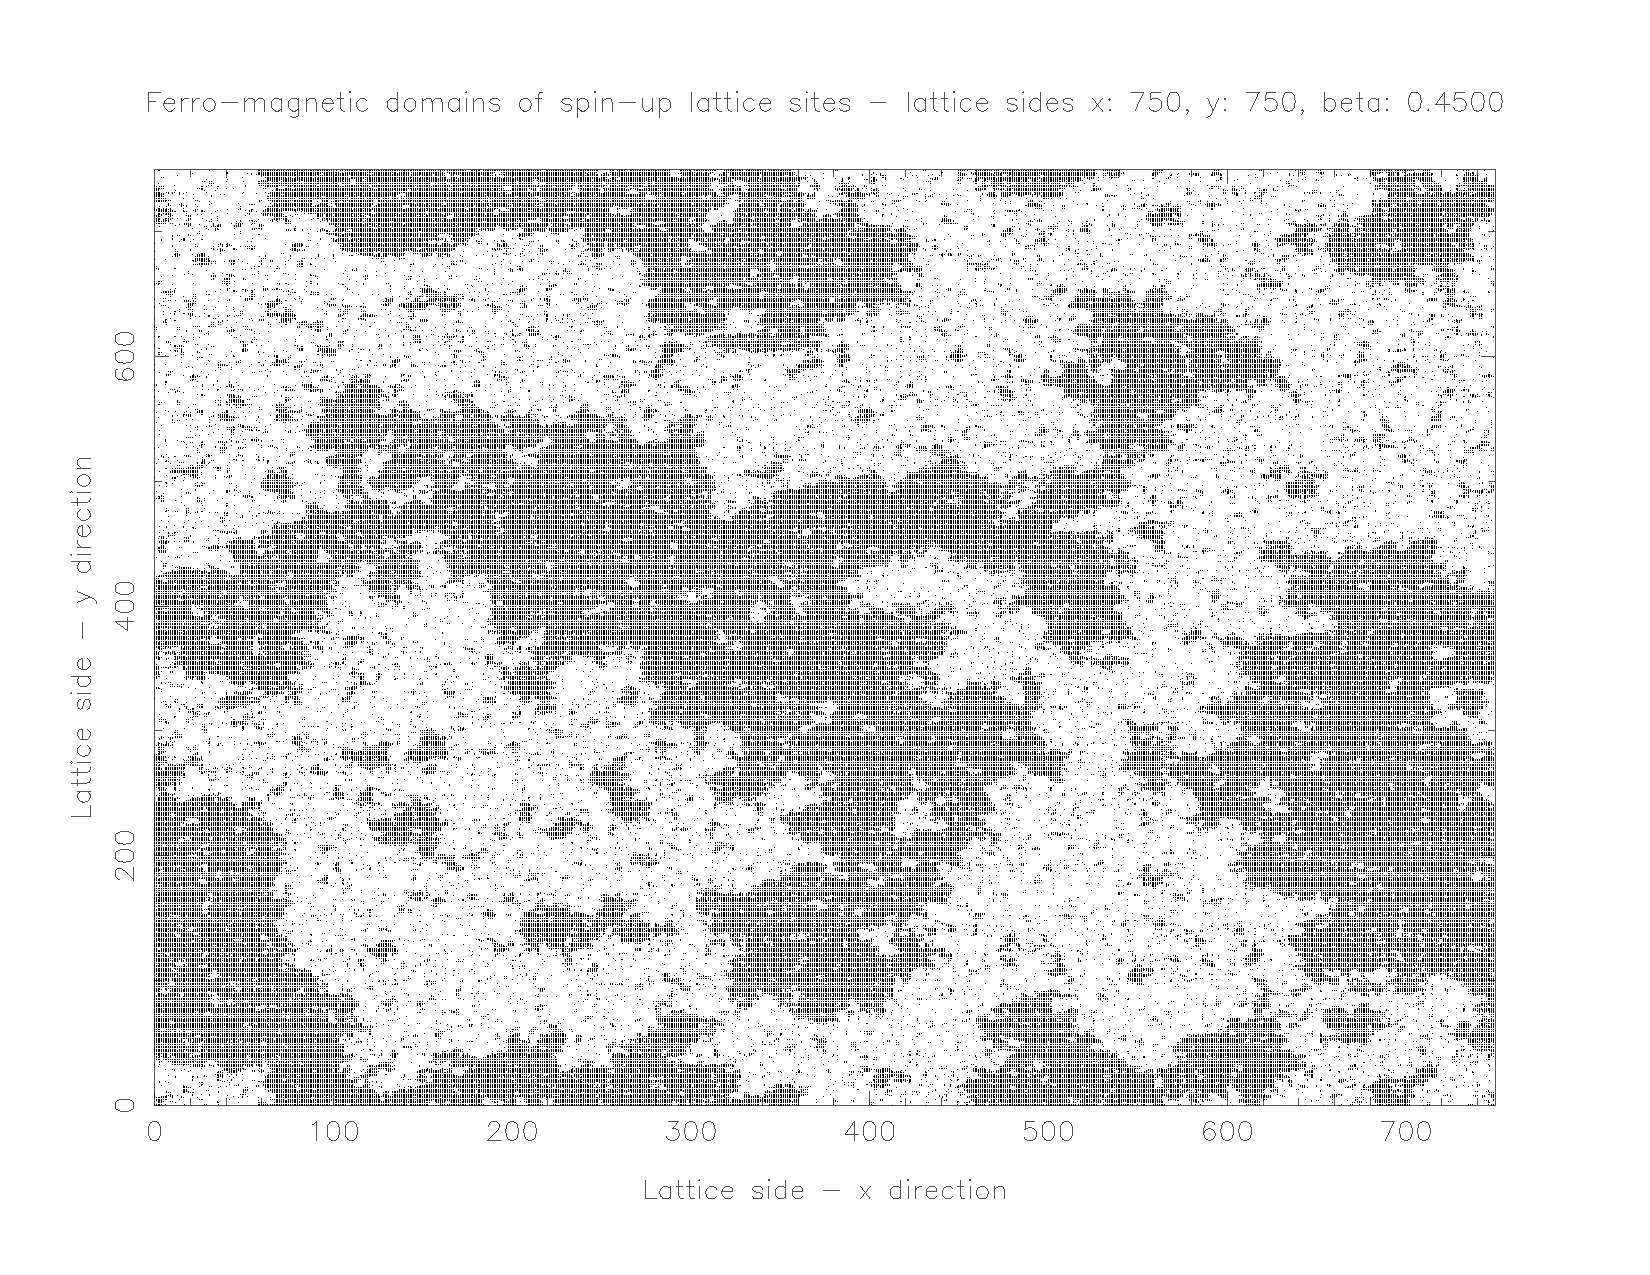
\includepdf[pages=1]{plots/proj4plot750.pdf}
	\caption{Scatter plot of lattice at $\beta\approx0.44$ showing ferro-magnetic domains.}\label{Fig_mag_plot_750_1}
\end{figure}

\clearpage
\begin{figure}[ht!]
	\centering
	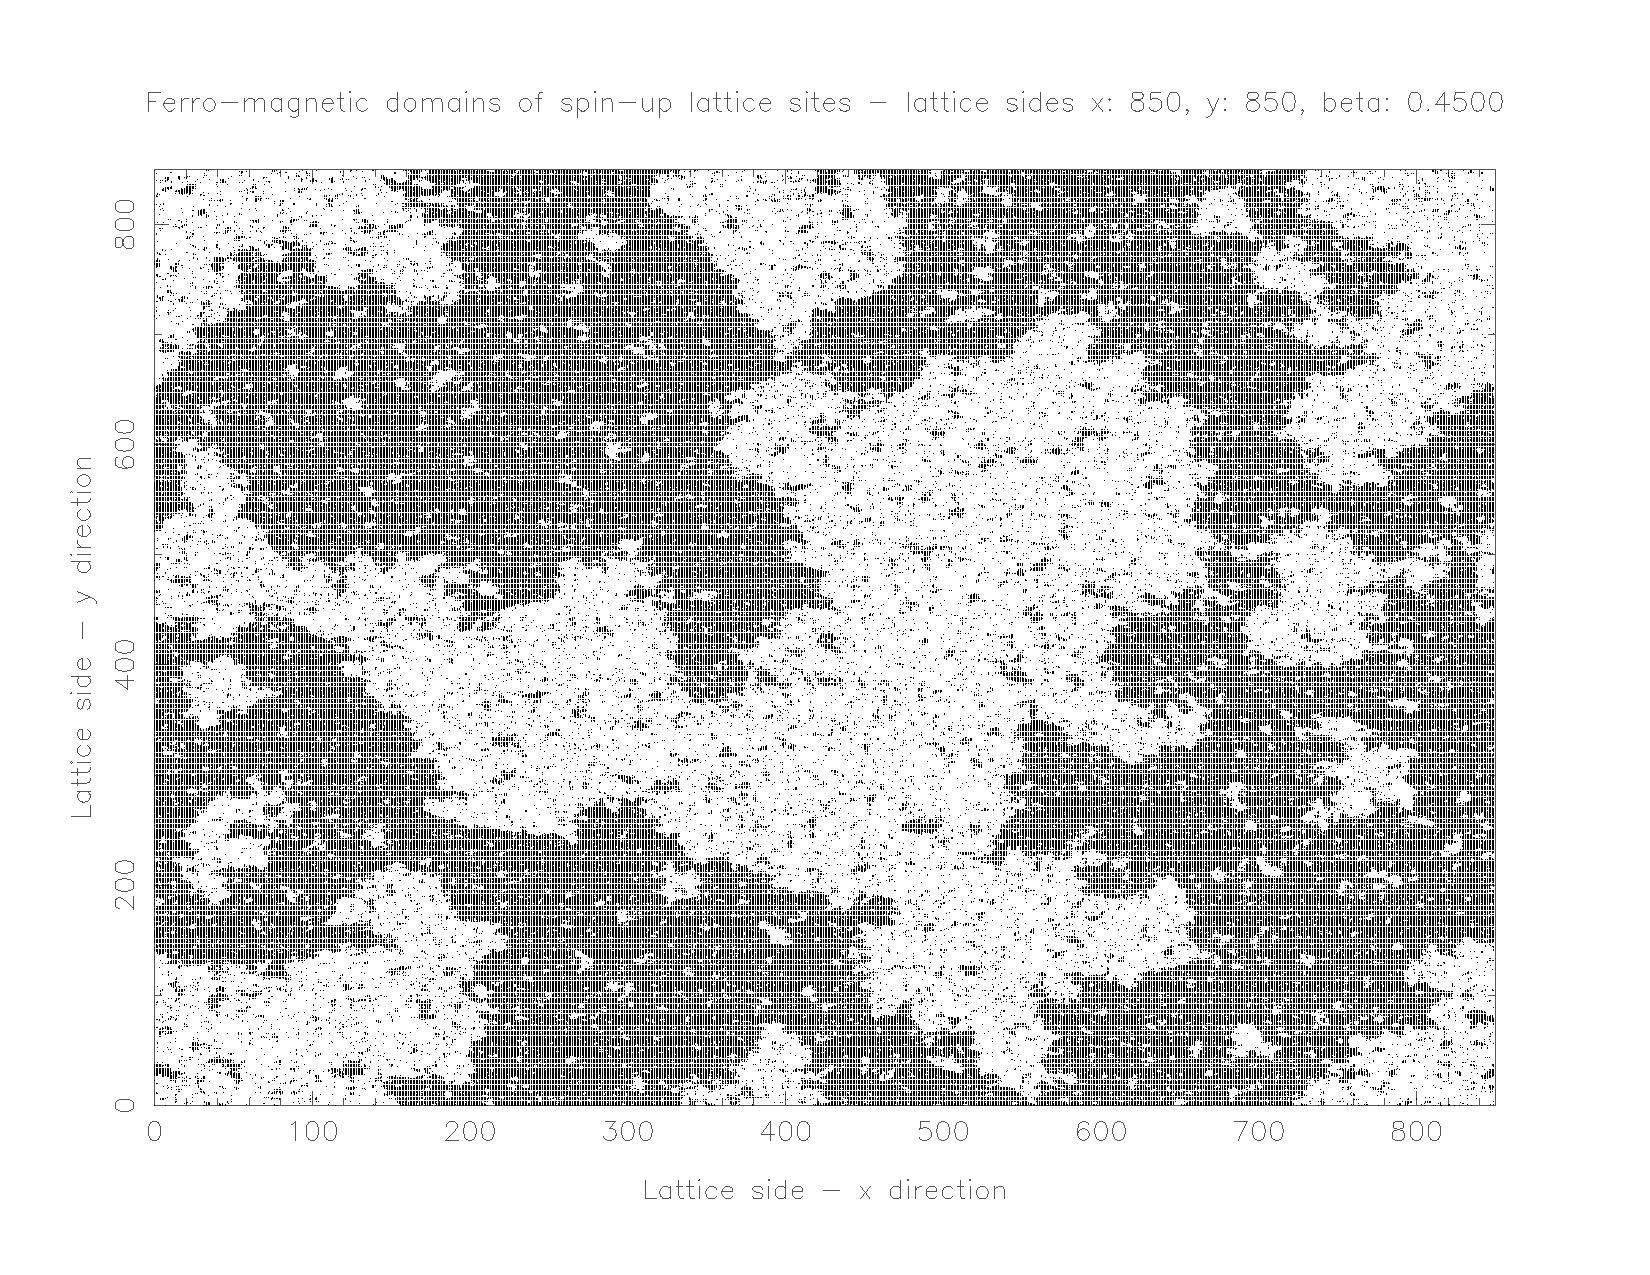
\includepdf[pages=1]{plots/proj4plot850.pdf}
	\caption{Scatter plot of lattice at $\beta\approx0.44$ showing ferro-magnetic domains.}\label{Fig_mag_plot_850_1}
\end{figure}

\clearpage
\begin{figure}[ht!]
	\centering
	\includepdf[pages=1]{plots/proj4plot1500.pdf}
	\caption{Scatter plot of lattice at $\beta\approx0.44$ showing ferro-magnetic domains.}\label{Fig_mag_plot_1500_1}
\end{figure}



\clearpage
\section{Conclusion}
We have created a program to implement the thermodynamic Ising model of a lattice as a 2D array of spins with simple nearest-neighbour interactions.\\

We have investigated the properties of this model and how the magnetisation changes with temperature for different lattice sizes. Specifically, we have noted that $\beta_c$ for the phase change in magnetisation is very similar to Onsager's analytic value in the large lattice limit.\\

For lattices larger than about 175x175, it is noted that an increase in the number of sweeps is required to thermalise the lattice in between measurements. We would expect this need to keep increasing with lattice size, and with sufficient computing resources this could be tested.\\

Also, we have demonstrated how up to a certain point, statistical errors can be controlled by adjusting the number of measurements, and systematic errors by altering the number of sweeps between each measurement and lattice size.

\begin{flushleft}
	\begin{thebibliography}{99}
			\bibitem{Manual}
			PHYC30012 Computational Physics manual
			\bibitem{Rand_v_syst_err}
			Exell R. H. B., \emph{Random vs Systematic Error}, viewed 10th Oct 2016, \textless http://www.jgsee.kmutt.ac.th/exell/PracMath/ErrorAn.htm \textgreater
			\bibitem{Syst_Wiki}
			Wikipedia, \emph{Observational error}, viewed 10th Oct 2016, \textless https://en.wikipedia.org/wiki/Observational\_error\#Systematic\_versus\_random\_error \textgreater
	\end{thebibliography}
\end{flushleft}

\end{document}